\documentclass[10pt,a4paper,notitlepage]{article}
%Mise en page
\usepackage[left=2cm, right=2cm, lines=45, top=0.8in, bottom=0.7in]{geometry}
\usepackage{fancyhdr}
\usepackage{fancybox}
\usepackage{pdfpages} 
\renewcommand{\headrulewidth}{1.5pt}
\renewcommand{\footrulewidth}{1.5pt}
\pagestyle{fancy}
\newcommand\Loadedframemethod{TikZ}
\usepackage[framemethod=\Loadedframemethod]{mdframed}
\usepackage{tikz}
\usetikzlibrary{calc,through,backgrounds}
\usetikzlibrary{matrix,positioning}
%Desssins geometriques
\usetikzlibrary{arrows}
\usetikzlibrary{shapes.geometric}
\usetikzlibrary{datavisualization}
\usetikzlibrary{automata} % LATEX and plain TEX
\usetikzlibrary{shapes.multipart}
\usetikzlibrary{decorations.pathmorphing} 
\usepackage{pgfplots}
\usepackage{physics}
\usepackage{titletoc}
\usepackage{mathpazo} 
\usepackage{algpseudocode}
\usepackage{algorithmicx} 
\usepackage{bohr} 
\usepackage{xlop} 
\usepackage{bbding} 
%\usepackage{minibox} 
%Ecriture arabe
\usepackage[french]{babel}
\usepackage[utf8]{inputenc}
\usepackage{mathdesign}
\usepackage{bbding} 
\usepackage{romande} 

\lhead{
\textbf{LU2PY013-PeiP }
}
\rhead{\textbf{03 mars 2020}
}
\chead{\textbf{
CC1
 }}

\lfoot{}
\cfoot{\textbf{$\mathsf{2019-2020}$}}
%\rfoot{\textit{Pr. $\mathcal{A}$.Kaal}}
%=====================Algo setup
\algblock{If}{EndIf}
\algcblock[If]{If}{ElsIf}{EndIf}
\algcblock{If}{Else}{EndIf}
\algrenewtext{If}{\textbf{si}}
\algrenewtext{Else}{\textbf{sinon}}
\algrenewtext{EndIf}{\textbf{finsi}}
\algrenewtext{Then}{\textbf{alors}}
\algrenewtext{While}{\textbf{tant que}}
\algrenewtext{EndWhile}{\textbf{fin tant que}}
\algrenewtext{Repeat}{\textbf{r\'ep\'eter}}
\algrenewtext{Until}{\textbf{jusqu'\`a}}
\algcblockdefx[Strange]{If}{Eeee}{Oooo}
[1]{\textbf{Eeee} "#1"}
{\textbf{Wuuuups\dots}}

\algrenewcommand\algorithmicwhile{\textbf{TantQue}}
\algrenewcommand\algorithmicdo{\textbf{Faire}}
\algrenewcommand\algorithmicend{\textbf{Fin}}
\algrenewcommand\algorithmicrequire{\textbf{Variables}}
\algrenewcommand\algorithmicensure{\textbf{Constante}}% replace ensure by constante
\algblock[block]{Begin}{End}
\newcommand\algo[1]{\textbf{algorithme} #1;}
\newcommand\vars{\textbf{variables } }
\newcommand\consts{\textbf{constantes}}
\algrenewtext{Begin}{\textbf{debut}}
\algrenewtext{End}{\textbf{fin}}
%================================
%================================

\setlength{\parskip}{1cm}
\setlength{\parindent}{1cm}
\tikzstyle{titregris} =
[draw=gray,fill=white, shading = exersicetitle, %
text=gray, rectangle, rounded corners, right,minimum height=.3cm]
\pgfdeclarehorizontalshading{exersicebackground}{100bp}
{color(0bp)=(green!40); color(100bp)=(black!5)}
\pgfdeclarehorizontalshading{exersicetitle}{100bp}
{color(0bp)=(red!40);color(100bp)=(black!5)}
\newcounter{exercise}
\renewcommand*\theexercise{exercice \textbf{Exercice}~n\arabic{exercise}}
\makeatletter
\def\mdf@@exercisepoints{}%new mdframed key:
\define@key{mdf}{exercisepoints}{%
\def\mdf@@exercisepoints{#1}
}
\mdfdefinestyle{exercisestyle}{%
outerlinewidth=1em,outerlinecolor=white,%
leftmargin=-1em,rightmargin=-1em,%
middlelinewidth=0.5pt,roundcorner=3pt,linecolor=black,
apptotikzsetting={\tikzset{mdfbackground/.append style ={%
shading = exersicebackground}}},
innertopmargin=0.1\baselineskip,
skipabove={\dimexpr0.1\baselineskip+0\topskip\relax},
skipbelow={-0.1em},
needspace=0.5\baselineskip,
frametitlefont=\sffamily\bfseries,
settings={\global\stepcounter{exercise}},
singleextra={%
\node[titregris,xshift=0.5cm] at (P-|O) %
{~\mdf@frametitlefont{\theexercise}~};
\ifdefempty{\mdf@@exercisepoints}%
{}%
{\node[titregris,left,xshift=-1cm] at (P)%
{~\mdf@frametitlefont{\mdf@@exercisepoints points}~};}%
},
firstextra={%
\node[titregris,xshift=1cm] at (P-|O) %
{~\mdf@frametitlefont{\theexercise}~};
\ifdefempty{\mdf@@exercisepoints}%
{}%
{\node[titregris,left,xshift=-1cm] at (P)%
{~\mdf@frametitlefont{\mdf@@exercisepoints points}~};}%
},
}
\makeatother


%%%%%%%%%

%%%%%%%%%%%%%%%
\mdfdefinestyle{theoremstyle}{%
outerlinewidth=0.01em,linecolor=black,middlelinewidth=0.5pt,%
frametitlerule=true,roundcorner=2pt,%
apptotikzsetting={\tikzset{mfframetitlebackground/.append style={%
shade,left color=white, right color=blue!20}}},
frametitlerulecolor=black,innertopmargin=1\baselineskip,%green!60,
innerbottommargin=0.5\baselineskip,
frametitlerulewidth=0.1pt,
innertopmargin=0.7\topskip,skipabove={\dimexpr0.2\baselineskip+0.1\topskip\relax},
frametitleaboveskip=1pt,
frametitlebelowskip=1pt
}
\setlength{\parskip}{0mm}
\setlength{\parindent}{10mm}
\mdtheorem[style=theoremstyle]{definition}{\textbf{Exercice}}
%================Liste definition--numList-and alphList=============
\newcounter{alphListCounter}
\newenvironment
{alphList}
{\begin{list}
{\alph{alphListCounter})}
{\usecounter{alphListCounter}
\setlength{\rightmargin}{0cm}
\setlength{\leftmargin}{0.5cm}
\setlength{\itemsep}{0.2cm}
\setlength{\partopsep}{0cm}
\setlength{\parsep}{0cm}}
}
{\end{list}}
\newcounter{numListCounter}
\newenvironment
{numList}
{\begin{list}
{\arabic{numListCounter})}
{\usecounter{numListCounter}
\setlength{\rightmargin}{0cm}
\setlength{\leftmargin}{0.5cm}
\setlength{\itemsep}{0cm}
\setlength{\partopsep}{0cm}
\setlength{\parsep}{0cm}}
}
{\end{list}}
%===========================================================
\begin{document}

\begin{center}
\large{\textbf{Corrigé}}
\end{center}
\begin{definition}[]
\hspace{0ex}\textbf{(30')} - Calculer les intégrales suivantes et préciser en une phrase si elles sont généralisées ou non :
\begin{enumerate}
   \item ${\displaystyle \int_0^1 x^2 \mathrm{ln}(x) dx}$ 
   
   \begin{center}
   En intégrant par partie,
   \begin{align*}
   \int_0^1 x^2 \mathrm{ln}(x) dx = \left[\dfrac{x^3}{3} \mathrm{ln}(x)\right]_0^1 - \int_0^1 \dfrac{x^2}{3}dx   =-\left[\dfrac{x^3}{9}\right]_0^1 =-\dfrac{1}{9}
   \end{align*}
   L'intégrale n'est pas généralisée car $\lim_{x \to 0} \left(x^2 \mathrm{ln}(x)\right)= 0$ par croissance comparée, la fonction est bien bornée sur le domaine d'intégration.
   \end{center}
   \item ${\displaystyle \int_0^{\pi/2} \dfrac{\cos(x)}{\sqrt{1+3\sin(x)}}dx}$
   \begin{center}
   En posant le changement de variable $y^2=1+3\sin(x)$, qui est bien bijectif sur l'intervalle considéré, alors $2y\mathrm{d}y=3\cos(x)dx$ et les nouvelles bornes vont de $y=1$ à $y=2$.
   \begin{align*}
   \int_0^{\pi/2} \dfrac{\cos(x)}{\sqrt{1+3\sin(x)}}dx = \int_1^2 \dfrac{\dfrac{2}{3}y\mathrm{d}y}{\sqrt{y^2}}=\int_1^2 \dfrac{2}{3}dy=\dfrac{2}{3}
   \end{align*}
   L'intégrale n'est pas généralisée.
   \end{center}
   \item  ${\displaystyle \int_{-\pi/2}^{\pi/2} \dfrac{\cos(x)-1}{\sin^2(x)}dx}$
   \begin{center}
   En remarquant que $$\dfrac{\mathrm{d}(1/\sin(x))}{dx}=-\dfrac{\cos(x)}{\sin^2(x)}$$
   Et que $$ \dfrac{1}{\sin^2(x)}=\dfrac{\sin^2(x)+\cos^2(x)}{\sin^2(x)}=1+\mathrm{cotan}^2(x)=-\mathrm{cotan}'(x)$$
   Il vient que $$\int_{-\pi/2}^{\pi/2} \dfrac{\cos(x)-1}{\sin^2(x)}dx = \left[-\dfrac{1}{\sin(x)}+\mathrm{cotan}(x)\right]_{-\pi/2}^{\pi/2} =\left[\dfrac{\cos(x)-1}{\sin(x)}\right]_{-\pi/2}^{\pi/2}=-2$$
   L'intégrale n'est pas généralisée car $\lim_{x \to 0}\left(\dfrac{\cos(x)-1}{\sin^2(x)}\right)=-\dfrac{1}{2}$ par les développement limités de $\sin^2(x)$ et $\cos(x) -1$ en $0$. La fonction est bien bornée sur son domaine d'intégration.
   \end{center}
\end{enumerate}
\end{definition}
%----------------
\begin{definition}
\hspace{0ex} \textbf{(15')} - Calcul de volumes en utilisant des intégrales simples :

\subsection*{Le cylindre}
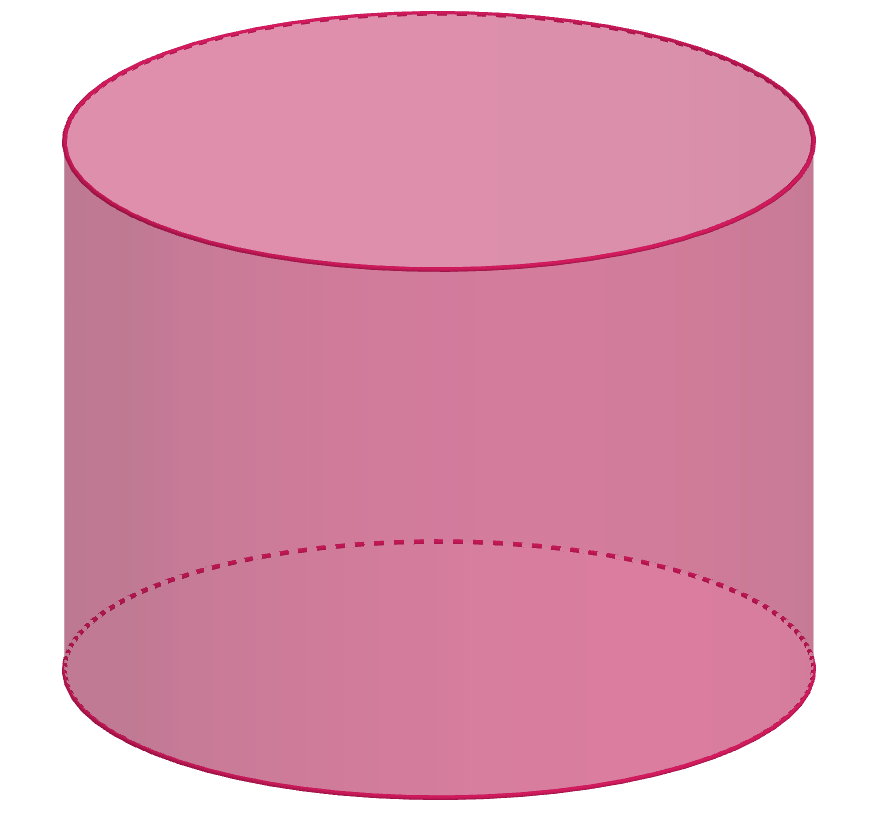
\includegraphics[scale=.15]{cylindre}

Le cylindre est un objet formidable (observez la figure ci dessus si vous ne nous croyez pas), surtout lorsqu'il a un rayon R et une hauteur h. La valeur de son volume va vous étonner ! Calculez-la en utilisant une intégrale simple. (Pour ce faire, vous vous rappelerez, avec nostalgie, l'équation d'un cercle de rayon R : $x^2+y^2=R^2$).


\subsection*{La toupie}
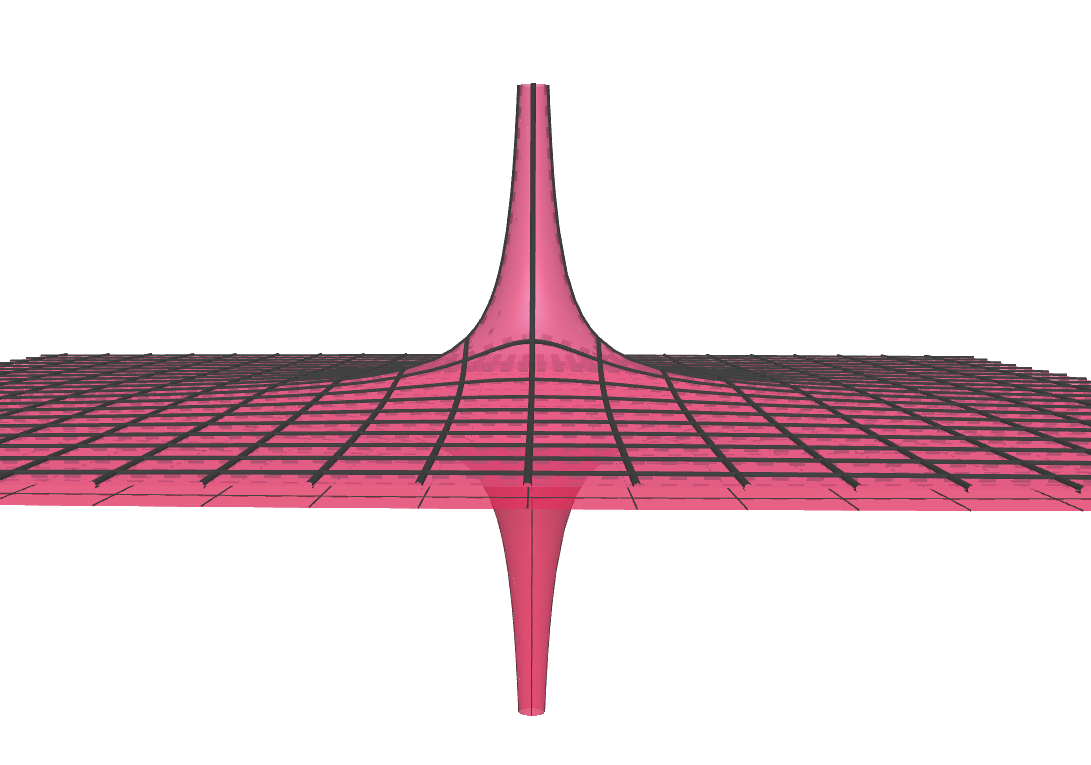
\includegraphics[scale=.15]{toupie}

Les toupies ne sont pas mal non plus. Celle-ci possède le petit désavantage d'être infinie. Mais son équation cartésienne est plutôt lisible :


\begin{equation*}
\left\{ 
        \begin{array}{rl}
    x^2+y^2&=\frac{1}{\sqrt{\abs{z}}}\\
    \abs{z}&\leq 5
    \end{array}
    \right.
\end{equation*}
Trouvez la valeur du volume de cette toupie (que vous pouvez admirer sur la figure ci dessus) en utilisant une intégrale simple.


\end{definition}
%----------------
\begin{definition}[]
%-- begin{minipage}{0.7\textwidth}
\hspace{0ex} \textbf{(10')} - Soit
%--\newline
\begin{equation}
y'(x)+\sin (x) y = \dfrac{e^{\cos(x)}}{\cos^2 (x)}
\end{equation}
\begin{enumerate}
\item Est-ce une équation différentielle linéaire ? (justifiez). De quel ordre ? (justifiez)
\item Résoudre cette équation sur un intervalle que l'on précisera (le plus grand possible).
\end{enumerate}

%--\end{minipage}
\end{definition}
%----------------
\begin{definition}[]
\textbf{(20')} - On cherche les fonctions y, solutions de :
\begin{equation}
\label{Eq2.2}
\dfrac{dy}{dx}e^{-y^2}(1-2y)=2xe^{-y}
\end{equation}
et vérifiant $y(1)=1$.
\begin{enumerate}
\item Est-ce que (\ref{Eq2.2}) est une équation différentielle linéaire ? (justifiez). De quel ordre ? (justifiez)
\item Calculer la dérivée de $e^{y(1-y)}$
\item Donner une EDO équivalente à (\ref{Eq2.2}) en utilisant la dérivée de $e^{y(1-y)}$ calculée juste avant. L'intégrer sur un intervalle que l'on précisera (le plus grand possible).
\end{enumerate}

%-\end{minipage}

\end{definition}
%----------------
\begin{definition}[]
\subsection*{(15') - Une balade en voiture en guise de dessert  }
\subsubsection*{- À l'arrêt }
La suspension d'une voiture de masse $m$ = 800 kg est équivalente à un ressort vertical de constante de raideur $k$ = 1,36 10$^4$ N/m, qui est associé à un frottement visqueux de constante $f$ = 1,6 10$^2$ kg/s.

L'équation du déplacement vertival $y(t)$ de la voiture s'écrit :

\begin {equation}
\quad  \quad \quad \quad \quad \quad \quad \quad \quad m\frac{d^{2}y}{dt^{2}}+f \frac{dy}{dt} +ky = 0
\end{equation}

\begin{enumerate}
   \item Cette équation différentielle est-elle linéaire ? Si oui, de quel ordre est-elle ? 
   \item Résoudre cette équation différentielle
\end{enumerate}
\subsubsection*{- Sur une route "ondulée"}
 On suppose maintenant que la voiture roule sur piste "ondulée" qui force une oscillation verticale de pulsation $\sqrt{17}$ et transforme l'équation différentielle initiale en :
\begin {equation}
\quad  \quad \quad \quad \quad \quad \quad m\frac{d^{2}y}{dt^{2}}+f \frac{dy}{dt} +ky = F\text{cos} \sqrt{17}t
\end{equation}
avec $F$= 800 N
\begin{enumerate}
   \item Simplifier cette équation différentielle en effectuant les applications numériques.
   \item Donner la solution générale en précisant l'intervalle de définition de $t$.
   \item Déterminer la solution particulière alors associée aux conditions initiales $y(t=0)=1$ et $y'(t=0) = -1$.
 
\end{enumerate}
\end{definition}



%% Macros for ``successive divisions'' 
%%
%\def\Division#1#2#3{ % Dividend, divisor, remainder
% \matrix (D) [matrix of nodes,
%              below=0pt of D-1-2.south east,
%              row sep=1pt, column sep=1pt,
%              every node/.append style={minimum width=12mm}] {
%   #1 \pgfmatrixnextcell #2 \\
%   |[marcar] (R#1)| #3      \\
% };
% \draw[shorten >=2pt, shorten <=2pt]
%   (D-1-2.north west) |- (D-1-2.south east);
%}
%\def\FinDivision#1{
%\node[marcar, below=2pt of D-1-2.south] (C)(C)  {#1};
%}
%\tikzset{marcar/.style={circle,draw,inner sep=2pt,minimum width=0pt,
%fill=yellow!10}}
%
%
%\begin{tikzpicture}
%  \coordinate (D-1-2) at (0,0) {}; % We must start with this command.
%  \Division{25}{2}{1} % First dividend, divisor, remainder
%  \Division{12}{2}{0} % Dividend (previous quotient), divisor, remainder
%  \Division{6}{2}{0}  
%  \Division{3}{2}{1}  
%  \FinDivision{1}     % Last remainder.
%
%% We can draw an arrow jumping from one remainder 
%% to the next one. Every reminder is a node called
%% Rdividend. Last remainder is node C.
%  \draw[shorten <=1mm, ->, dashed] (C) to[out=-150,in=-65] (R3);
%  \draw[shorten <=1mm, ->, dashed] (R3) to[out=-150,in=-65] (R6);
%  \draw[shorten <=1mm, ->, dashed] (R6) to[out=-150,in=-65] (R12);
%  \draw[shorten <=1mm, ->, dashed] (R12) to[out=-150,in=-65] (R25);
%
%% Some more information:
%  \node (MSB) at ([yshift=-1.3cm]R6.south) {Most significant bit (MSB)};    
%  \node (LSB) at ([yshift=-2mm]MSB.south) {Less significant bit (LSB)}; 
%\draw[ ->] (MSB.east) to[out=30,in=-55] (C);
%\draw[ ->] (LSB.west) to[out=150,in=-95] (R25);
%\end{tikzpicture}
%\begin{center}\SnowflakeChevronBold \SnowflakeChevronBold \SnowflakeChevronBold \end{center}
%%----------------------------------------------------------------------------------------------------------------------------------------
%
%%\includepdf[doublepages=true]{serie55}

\end{document}